% !TEX root = ../../main.tex
\chapter{Landasan Teori}

\section{Mobile Edge Computing dan Model Task Offloading}
\label{sec:mobile_edge_computing_dan_model_task_offloading}

\subsection{Konsep dan Arsitektur MEC}
\label{subsec:konsep_dan_arsitektur_mec}

Mobile Edge Computing (MEC) merupakan paradigma komputasi terdistribusi yang menempatkan sumber daya pemrosesan dan penyimpanan pada sisi jaringan, lebih dekat dengan perangkat pengguna. Berbeda dengan \textit{cloud computing} yang umumnya memusatkan pemrosesan pada pusat data, MEC memungkinkan tugas komputasi diproses melalui server yang berada di sekitar jaringan akses. Penempatan sumber daya tersebut bertujuan mengurangi jarak komunikasi antara perangkat dan lokasi pemrosesan sehingga dapat menekan latensi, khususnya untuk aplikasi yang membutuhkan respons cepat \cite{yousefpour2019all, mach2017mobile, mao2017survey}.

Secara umum, arsitektur MEC terdiri atas perangkat \textit{mobile} sebagai penghasil tugas komputasi, jaringan akses sebagai media komunikasi, dan \textit{edge node} sebagai penyedia sumber daya pemrosesan. Infrastruktur \textit{cloud} juga dapat digunakan sebagai lapisan komputasi tambahan, tetapi tidak menjadi bagian utama dari model sistem yang dibahas dalam penelitian ini. Penelitian ini berfokus pada interaksi antara sejumlah perangkat \textit{mobile} dan \textit{edge node} yang memiliki kapasitas komputasi terbatas. Ketika beberapa perangkat mengalihkan tugas ke \textit{edge node} yang sama, beban pemrosesan pada node tersebut dapat meningkat dan memengaruhi waktu penyelesaian tugas \cite{tang2022deep, mach2017mobile}.

Jaringan akses berfungsi sebagai media komunikasi antara perangkat \textit{mobile} dan \textit{edge node}. Teknologi akses dapat berupa jaringan seluler maupun Wi-Fi, bergantung pada implementasi sistem MEC. Dalam penelitian ini, jaringan akses direpresentasikan sebagai media komunikasi antara perangkat dan \textit{edge node}, tanpa membandingkan karakteristik teknologi akses tertentu. \textit{Edge node} menyediakan sumber daya pemrosesan bersama yang digunakan oleh sejumlah perangkat \textit{mobile} untuk menjalankan tugas komputasi yang dialihkan. Ilustrasi arsitektur sistem MEC dalam penelitian ini disajikan pada Gambar~\ref{fig:arsitektur_mec}.

\begin{figure}[H]
	\centering
	\includegraphics[width=0.75\textwidth]{\detokenize{picture/MEC Infrastructure_.png}}
	\caption{Arsitektur \textit{Mobile Edge Computing} dalam Penelitian}
	\label{fig:arsitektur_mec}
	\vspace{0.5ex}
	{\footnotesize Sumber: Diadaptasi dari \cite{tang2022deep} dan \cite{mach2017mobile}.}
\end{figure}

\vspace{1cm}
\subsection{Mekanisme Task Offloading dan Model Tugas}
\label{subsec:mekanisme_task_offloading_dan_model_tugas}

\textit{Task offloading} merupakan mekanisme pemindahan tugas komputasi dari perangkat pengguna ke sumber daya komputasi lain, seperti \textit{edge node}. Keputusan ini bertujuan mengatasi keterbatasan kapasitas pemrosesan perangkat dengan mempertimbangkan kondisi komputasi dan komunikasi. Secara umum, offloading dapat dilakukan secara penuh (\textit{full offloading}), yaitu seluruh tugas dialihkan, atau secara parsial (\textit{partial offloading}), yaitu tugas dibagi menjadi beberapa bagian untuk diproses pada lokasi berbeda \cite{acheampong2023review, mach2017mobile}.

Model yang digunakan oleh Tang dan Wong \cite{tang2022deep} mempertimbangkan tugas yang tidak dapat dibagi (\textit{non-divisible tasks}) dan sensitif terhadap keterlambatan (\textit{delay-sensitive tasks}). Dengan demikian, setiap tugas diproses secara lokal pada perangkat atau dialihkan secara utuh ke salah satu \textit{edge node}. Sistem terdiri atas himpunan perangkat $\mathcal{M}=\{1,2,\ldots,M\}$ dan himpunan \textit{edge node} $\mathcal{N}=\{1,2,\ldots,N\}$.

Tugas yang tiba pada perangkat $m$ di slot waktu $t$ memiliki ukuran data $\lambda_m(t)$ dalam bit, kepadatan komputasi $\rho_m$ dalam siklus CPU per bit, serta batas waktu penyelesaian (\textit{deadline}) $\tau_m$ dalam slot waktu. Oleh karena itu, kebutuhan komputasi tugas tersebut adalah:

\begin{equation}
\label{eq:kebutuhan_komputasi}
C_m(t)=\lambda_m(t)\rho_m
\end{equation}

\noindent dengan $C_m(t)$ menyatakan jumlah siklus CPU yang dibutuhkan untuk menyelesaikan tugas.

Keputusan pemrosesan direpresentasikan menggunakan variabel biner $x_m(t)$, sedangkan pemilihan \textit{edge node} tujuan dinyatakan dengan variabel $y_{m,n}(t)$:

\begin{equation}
\label{eq:keputusan_lokal}
x_m(t)=
\begin{cases}
1, & \text{jika tugas diproses secara lokal}\\
0, & \text{jika tugas dialihkan}
\end{cases}
\end{equation}

\begin{equation}
\label{eq:keputusan_offload}
y_{m,n}(t)=
\begin{cases}
1, & \text{jika tugas dialihkan ke edge node }n\\
0, & \text{lainnya}
\end{cases}
\end{equation}

Karena setiap tugas hanya dapat dialihkan ke satu \textit{edge node}, keputusan tersebut harus memenuhi:

\begin{equation}
\label{eq:kendala_offload}
\sum_{n\in\mathcal{N}}y_{m,n}(t)
=
\mathds{1}\big(x_m(t)=0\big)
\end{equation}

\noindent dengan $\mathds{1}(\cdot)$ merupakan fungsi indikator. Persamaan tersebut menunjukkan bahwa apabila tugas diproses secara lokal, tidak ada \textit{edge node} yang dipilih. Sebaliknya, apabila tugas dialihkan, tepat satu \textit{edge node} harus menjadi tujuan pemrosesan \cite{tang2022deep}. Model sistem dan alur mekanisme \textit{task offloading} tersebut diilustrasikan pada Gambar~\ref{fig:mekanisme_task_offloading}.

\begin{figure}[H]
	\centering
	\includegraphics[width=1.13\textwidth]{\detokenize{picture/TaskOffloadingMechanism.pdf}}
	\caption{Model Sistem dan Mekanisme \textit{Task Offloading} pada \textit{Mobile Edge Computing}}
	\label{fig:mekanisme_task_offloading}
	\vspace{0.5ex}
	{\footnotesize Sumber: Diadaptasi dari Tang dan Wong \cite{tang2022deep}.}
\end{figure}

\vspace{1cm}
\subsection{Model Antrean dan Kinerja Eksekusi Tugas}
\label{subsec:model_antrean_dan_kinerja_eksekusi_tugas}

Proses penyelesaian tugas pada MEC dipengaruhi oleh antrean dan kapasitas sumber daya pada setiap tahap pemrosesan. Dalam model Tang dan Wong \cite{tang2022deep}, terdapat tiga jenis antrean, yaitu antrean komputasi lokal, antrean transmisi, dan antrean komputasi pada \textit{edge node}. Ketiganya menggunakan \textit{First-In First-Out} (FIFO) sebagai model antriannya.

\textbf{Pertama, antrean komputasi lokal} menampung tugas yang diproses langsung oleh perangkat \textit{mobile}. Antrean ini dilayani oleh CPU perangkat dengan kapasitas pemrosesan $f_m^{\mathrm{device}}$. Waktu penyelesaian tugas dipengaruhi oleh jumlah pekerjaan yang masih menunggu dalam antrean dan kapasitas CPU perangkat tersebut.

\textbf{Kedua, antrean transmisi} menampung tugas yang dipilih untuk dialihkan ke \textit{edge node}. Tugas dikirimkan melalui jaringan nirkabel menggunakan antarmuka komunikasi perangkat. Dalam model tersebut, laju transmisi antara perangkat $m$ dan \textit{edge node} $n$ dinyatakan sebagai:

\begin{equation}
\label{eq:laju_transmisi}
r_{m,n}^{\mathrm{tran}}
=
W\log_2
\left(
1+\frac{|h_{m,n}|^2P}{\sigma^2}
\right)
\end{equation}

%Teorema Shannon-Hartley adalah hukum fundamental dalam teori informasi dan telekomunikasi 
%yang menetapkan batas kecepatan maksimum suatu data dapat dikirimkan secara bebas kesalahan melalui saluran komunikasi yang memiliki derau (noise)
% NOTE / CATATAN:
% Rumus di dalam kurung (|h_{m,n}|^2 P / \sigma^2) disebut sebagai SNR (Signal-to-Noise Ratio).
% Intinya: Seberapa kuat sinyal yang diterima dibandingkan dengan gangguan bisingnya.
% Jika sinyal kuat dan bising kecil, SNR tinggi, maka laju transmisi (r) akan semakin cepat.

\noindent dengan $W$ merupakan bandwidth kanal, $h_{m,n}$ adalah koefisien kanal komunikasi, $P$ merupakan daya transmisi, dan $\sigma^2$ adalah daya \textit{noise} pada penerima. Berdasarkan persamaan tersebut, waktu pengiriman dipengaruhi oleh ukuran tugas dan kondisi kanal komunikasi. Selain waktu transmisi, tugas juga dapat mengalami waktu tunggu sebelum memperoleh giliran untuk dikirimkan \cite{tang2022deep}.

\textbf{Ketiga, antrean komputasi pada edge node} menampung tugas yang telah berhasil dikirimkan dari perangkat \textit{mobile}. Dalam model Tang dan Wong \cite{tang2022deep}, setiap \textit{edge node} memiliki antrean FIFO untuk masing-masing perangkat \textit{mobile}. Antrean yang sedang berisi tugas atau menerima kedatangan tugas pada slot waktu tertentu dikategorikan sebagai antrean aktif. Seluruh antrean aktif pada satu \textit{edge node} berbagi kapasitas CPU menggunakan mekanisme \textit{Generalized Processor Sharing} (GPS) dengan bobot layanan yang sama.

Misalkan $\mathcal{B}_n(t)$ merupakan himpunan antrean aktif pada \textit{edge node} $n$, sedangkan $B_n(t)$ merupakan jumlah antrean aktif tersebut:

\begin{equation}
\label{eq:jumlah_antrean_aktif}
B_n(t)=|\mathcal{B}_n(t)|
\end{equation}

Apabila kapasitas CPU \textit{edge node} $n$ adalah $f_n^{\mathrm{edge}}$, kapasitas yang dialokasikan kepada setiap antrean aktif dinyatakan sebagai:

\begin{equation}
\label{eq:alokasi_cpu_edge}
f_{m,n}^{\mathrm{allocated}}(t)
=
\frac{f_n^{\mathrm{edge}}}{B_n(t)}
\end{equation}

Pembagian ini menunjukkan bahwa kapasitas komputasi yang diterima setiap antrean bergantung pada jumlah antrean aktif. Ketika jumlah antrean meningkat, bagian kapasitas CPU yang tersedia bagi setiap antrean menjadi lebih kecil. Akibatnya, waktu tunggu dan waktu pemrosesan tugas dapat meningkat \cite{tang2022deep}.

Secara keseluruhan, \textit{task processing delay} merupakan durasi sejak tugas tiba hingga selesai diproses. Pada pemrosesan lokal, durasi tersebut mencakup waktu tunggu dan waktu eksekusi pada perangkat. Sementara itu, pada mekanisme offloading, durasi mencakup waktu tunggu transmisi, pengiriman melalui jaringan, waktu tunggu pada antrean \textit{edge node}, serta waktu pemrosesan di \textit{edge node}. Apabila tugas tiba pada slot $t$ dan selesai pada slot $t_m^{\mathrm{finish}}(t)$, durasi penyelesaiannya dapat dinyatakan sebagai:

\begin{equation}
\label{eq:durasi_penyelesaian_tugas}
D_m(t)=t_m^{\mathrm{finish}}(t)-t+1
\end{equation}

Setiap tugas memiliki \textit{deadline} $\tau_m$. Apabila tugas belum selesai diproses hingga akhir slot $t+\tau_m-1$, tugas tersebut dinyatakan mengalami \textit{task dropping}. Dengan demikian, keterbatasan kapasitas komputasi, antrean yang padat, maupun kondisi transmisi dapat menyebabkan tugas tidak selesai sebelum batas waktu yang ditentukan.

Dalam formulasi Tang dan Wong \cite{tang2022deep}, tugas yang berhasil diproses menghasilkan biaya (\textit{cost}) sebesar waktu penyelesaiannya, sedangkan tugas yang mengalami \textit{dropping} dikenai penalti konstan $C>0$. Formulasi ini digunakan untuk membedakan konsekuensi antara tugas yang berhasil diselesaikan dan tugas yang gagal memenuhi \textit{deadline}. Pembahasan mengenai penggunaan \textit{cost} sebagai tujuan pembelajaran serta metrik evaluasinya dijelaskan pada bagian selanjutnya.

\vspace{1cm}
\section{Beban Kerja Non-Stasioner}
\label{sec:beban_kerja_non_stasioner}

Dalam sistem MEC, \textit{workload} menggambarkan proses kedatangan tugas yang harus ditangani oleh perangkat dan \textit{edge node}. Karakteristiknya dapat berubah sepanjang waktu dan memengaruhi kondisi lingkungan tempat agen melakukan pembelajaran. Berdasarkan kestabilan karakteristik statistiknya, workload dapat dibedakan menjadi \textit{stationary} dan \textit{non-stationary} \cite{tang2022deep, padakandla2020reinforcement}.

\vspace{1cm}
\subsection{Stationary dan Non-Stationary Workload}
\label{subsec:stationary_dan_non_stationary_workload}

\textit{Stationary workload} merupakan kondisi ketika mekanisme statistik pembangkit workload tetap sepanjang waktu. Kedatangan tugas tetap dapat berubah secara acak pada setiap slot, tetapi distribusi dan karakteristik temporal yang mendasarinya tidak berubah. Sebaliknya, \textit{non-stationary workload} terjadi ketika distribusi atau parameter pembangkit workload berubah seiring waktu \cite{padakandla2020reinforcement, khetarpal2022towards}.

Perbedaan tersebut dapat dinyatakan sebagai berikut:

\begin{equation}
\label{eq:stationary_vs_nonstationary}
\begin{aligned}
\text{Stationary:}\quad
&p(t)=p_0,\quad \forall t\\
\text{Non-stationary:}\quad
&\exists\,t_1,t_2:\ p(t_1)\neq p(t_2)
\end{aligned}
\end{equation}

Dalam penelitian ini, $p(t)$ merepresentasikan probabilitas kedatangan tugas pada slot waktu $t$ dalam generator \textit{workload} simulator. Persamaan tersebut digunakan untuk menggambarkan perubahan parameter probabilitas kedatangan pada skenario pengujian. Namun, perubahan nilai probabilitas pada suatu lintasan tidak selalu berarti bahwa proses stokastik yang mendasarinya bersifat nonstasioner. Khusus pada proses \textit{Markov-modulated}, sifat stasioner secara formal juga bergantung pada distribusi awal dan matriks transisi rezim yang digunakan.

Dalam Reinforcement Learning, perubahan workload dapat memengaruhi distribusi \textit{state} yang dialami agen serta dinamika transisi dan biaya yang dihasilkan lingkungan. Akibatnya, kebijakan yang dipelajari pada kondisi sebelumnya berpotensi tidak lagi optimal ketika karakteristik workload berubah \cite{padakandla2020reinforcement}.

\vspace{1cm}
\subsection{Distribution Shift dan Dampaknya pada Independent Learners}
\label{subsec:distribution_shift}

\textit{Distribution shift} dalam penelitian ini merujuk pada perubahan distribusi workload yang menyebabkan kondisi lingkungan yang dihadapi agen berbeda dari kondisi sebelumnya. Dalam formulasi RL, perubahan tersebut dapat memengaruhi probabilitas transisi \textit{state} maupun distribusi biaya:

\begin{equation}
\label{eq:perubahan_transisi_state}
P_t(s'\mid s,a)\neq P_{t'}(s'\mid s,a)
\end{equation}

atau

\begin{equation}
\label{eq:perubahan_distribusi_biaya}
p_t(c\mid s,a)\neq p_{t'}(c\mid s,a)
\end{equation}

dengan $s$ merupakan \textit{state}, $a$ adalah tindakan, dan $c$ menyatakan biaya yang diterima agen. Perubahan ini dapat menyebabkan kebijakan yang sebelumnya efektif menghasilkan keputusan yang kurang sesuai pada kondisi workload baru \cite{padakandla2020reinforcement}.

Pada sistem MEC terdistribusi, setiap perangkat \textit{mobile} menjalankan agen independen (\textit{independent learner}) berdasarkan observasi lokal. Meskipun agen tidak bertukar kebijakan secara langsung, penggunaan \textit{edge node} secara bersama menyebabkan keputusan setiap perangkat dapat memengaruhi tingkat antrean dan kapasitas komputasi yang tersedia bagi perangkat lainnya \cite{tang2022deep}.

Selain perubahan workload eksternal, pembaruan kebijakan agen lain selama pembelajaran juga dapat menimbulkan nonstasioneritas dari sudut pandang \textit{independent learner} \cite{papoudakis2019dealing}. Penelitian ini memusatkan evaluasi pada perubahan workload eksternal, sementara interaksi antaragen melalui penggunaan sumber daya bersama tetap menjadi bagian dari dinamika sistem.

\vspace{1cm}
\subsection{Pola Perubahan Workload}
\label{subsec:pola_perubahan_workload}

Penelitian ini menggunakan dua kondisi stasioner sebagai pembanding dan empat pola workload yang merepresentasikan karakteristik perubahan berbeda.


\begin{table}[H]
\centering
\caption{Karakteristik Workload yang Digunakan dalam Penelitian}
\label{tab:pola_perubahan_workload}
\renewcommand{\arraystretch}{1.3}
\begin{tabularx}{\textwidth}{c l X}
\toprule
\textbf{No.} & \textbf{Skenario} & \textbf{Karakteristik} \\
\midrule
1 & \textit{Stationary Baseline}
  & Beban kerja dengan probabilitas kedatangan yang tetap secara statistik sepanjang simulasi. \\

2 & \textit{Stationary Control}
  & Beban kerja stasioner dengan probabilitas kedatangan tetap yang digunakan sebagai kondisi pembanding terhadap \textit{Sudden Shift}, dengan rata-rata probabilitas kedatangan yang setara. \\

3 & \textit{Sudden Shift}
  & Perubahan intensitas kedatangan tugas secara mendadak dari satu kondisi beban kerja ke kondisi lainnya. \\

4 & \textit{Sinusoidal Diurnal Wave}
  & Perubahan intensitas kedatangan tugas secara periodik mengikuti pola gelombang sinusoidal. \\

5 & \textit{Bursty / Flash Crowd Spikes}
  & Lonjakan kedatangan tugas dalam interval tertentu dengan intensitas tinggi, yang diselingi periode dengan intensitas lebih rendah. \\

6 & \textit{Markov-Modulated Workload}
  & Pola kedatangan tugas yang dipengaruhi oleh kondisi atau rezim workload yang berubah mengikuti proses Markov. \\
\bottomrule
\end{tabularx}
\end{table}

Pada pola \textit{Markov-Modulated Workload}, kondisi beban kerja direpresentasikan menggunakan variabel $z_t$ yang menunjukkan rezim workload aktif pada waktu $t$. Perpindahan antarkondisi mengikuti probabilitas transisi Markov:

\begin{equation}
\label{eq:transisi_rezim_markov}
P(z_t=j\mid z_{t-1}=i)=q_{ij}
\end{equation}

dengan $q_{ij}$ merupakan probabilitas perpindahan dari rezim $i$ ke rezim $j$. Probabilitas kedatangan tugas bergantung pada rezim yang sedang aktif, sehingga dapat dinyatakan sebagai:

\begin{equation}
\label{eq:probabilitas_arrival_markov}
p(t)=p_{z_t}
\end{equation}

Mekanisme tersebut menghasilkan variasi intensitas kedatangan tugas berdasarkan perpindahan kondisi workload secara stokastik.

Keenam profil tersebut digunakan untuk mengevaluasi respons agen LSTM-D3QN terhadap kondisi workload yang berbeda. Dua profil stasioner berfungsi sebagai kondisi pembanding, sedangkan empat profil lainnya merepresentasikan variasi dinamika kedatangan tugas. Rincian implementasi dan parameter pembangkitan setiap profil workload dijelaskan pada Bab III.

\vspace{1cm}
\section{Reinforcement Learning}
\label{sec:reinforcement_learning}

\textit{Reinforcement Learning} (RL) merupakan paradigma pembelajaran mesin yang memungkinkan agen mempelajari strategi pengambilan keputusan melalui interaksi dengan lingkungan. Agen mengamati kondisi lingkungan, memilih tindakan, dan menerima umpan balik berdasarkan konsekuensi tindakan tersebut. Pengalaman dari interaksi berulang digunakan untuk memperbaiki kebijakan pengambilan keputusan agar tujuan pembelajaran dapat dicapai dalam jangka panjang \cite{suttonbarto2018}.

Sutton dan Barto \cite{suttonbarto2018} merumuskan tujuan RL sebagai maksimisasi ekspektasi akumulasi \textit{reward}. Sementara itu, penelitian ini menggunakan formulasi minimisasi \textit{cost} sesuai dengan permasalahan \textit{task offloading} pada MEC. Kedua formulasi tersebut memiliki prinsip optimasi yang ekuivalen melalui transformasi tanda antara \textit{reward} dan \textit{cost}.

\vspace{1cm}
\subsection{Interaksi Agen-Lingkungan dan Formulasi MDP}
\label{subsec:interaksi_agen_lingkungan_mdp}

Interaksi dalam RL berlangsung antara agen (\textit{agent}) dan lingkungan (\textit{environment}). Pada setiap langkah waktu $t$, agen menerima informasi kondisi lingkungan yang dinyatakan sebagai \textit{state} $S_t$, kemudian memilih tindakan $A_t$. Lingkungan merespons tindakan tersebut dengan menghasilkan umpan balik berupa \textit{reward} $R_{t+1}$ dan kondisi berikutnya $S_{t+1}$. Proses ini berlangsung secara berulang dan membentuk pengalaman yang digunakan agen dalam pembelajaran. Mekanisme interaksi tersebut ditunjukkan pada Gambar~\ref{fig:agent_environment} \cite{suttonbarto2018}.

\begin{figure}[H]
    \centering
    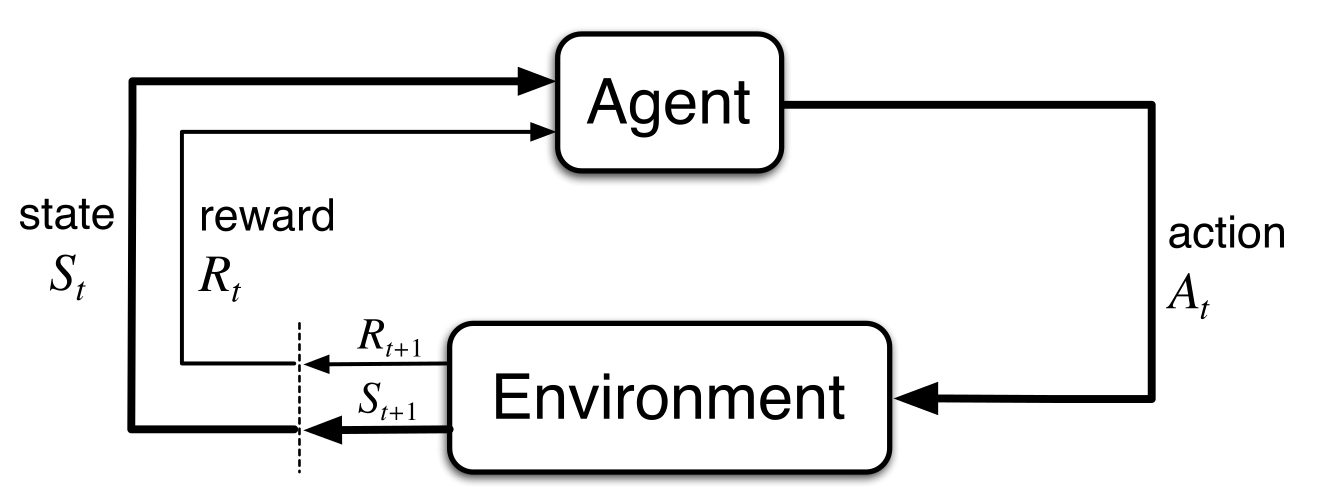
\includegraphics[width=0.75\textwidth]{picture/AgentEnvironment.png}
    \caption{Interaksi Agen dan Lingkungan dalam Markov Decision Process}
    \label{fig:agent_environment}
    \vspace{0.5ex}
    {\footnotesize Sumber: Sutton dan Barto \cite[hlm.~48]{suttonbarto2018}.}
\end{figure}

Interaksi agen dan lingkungan dapat diformulasikan menggunakan \textit{Markov Decision Process} (MDP), yaitu kerangka matematis untuk merepresentasikan pengambilan keputusan berdasarkan kondisi, tindakan, dan konsekuensinya. Dinamika lingkungan dalam MDP dinyatakan melalui probabilitas transisi:

\begin{equation}
\label{eq:mdp_transition}
p(s',r\mid s,a)
=
\Pr\{S_{t+1}=s',R_{t+1}=r
\mid S_t=s,A_t=a\}
\end{equation}

dengan $s$ dan $s'$ menyatakan \textit{state} saat ini dan berikutnya, $a$ merupakan tindakan yang dipilih agen, sedangkan $r$ merupakan \textit{reward} yang diterima. Fungsi tersebut menggambarkan probabilitas lingkungan menghasilkan kondisi berikutnya beserta \textit{reward} berdasarkan kondisi dan tindakan saat ini \cite{suttonbarto2018}.

MDP memiliki sifat Markov (\textit{Markov property}), yaitu probabilitas kondisi dan umpan balik berikutnya hanya bergantung pada \textit{state} dan tindakan saat ini, bukan pada keseluruhan riwayat interaksi sebelumnya. Sifat tersebut dinyatakan sebagai:

\begin{equation}
\label{eq:markov_property}
\begin{aligned}
&\Pr(S_{t+1}=s',R_{t+1}=r
\mid \mathcal{H}_t,S_t=s,A_t=a)\\
&\qquad =p(s',r\mid s,a)
\end{aligned}
\end{equation}

dengan $\mathcal{H}_t$ menyatakan riwayat interaksi sebelum waktu $t$. Oleh karena itu, \textit{state} harus memuat informasi yang relevan untuk menggambarkan dinamika lingkungan berikutnya \cite{suttonbarto2018}.

Dalam simulator penelitian ini, kedatangan tugas pada setiap perangkat dimodelkan menggunakan variabel Bernoulli. Indikator kedatangan tugas pada perangkat $m$ di slot waktu $t$ dinyatakan sebagai:

\begin{equation}
\label{eq:bernoulli_arrival}
I_m(t)\sim \operatorname{Bernoulli}(p(t))
\end{equation}

dengan $I_m(t)=1$ menunjukkan adanya tugas baru, sedangkan $I_m(t)=0$ menunjukkan tidak ada kedatangan tugas. Parameter $p(t)$ merupakan probabilitas kedatangan tugas pada slot waktu $t$. Pada kondisi stasioner, nilai probabilitas tersebut tetap, sedangkan pada kondisi nonstasioner nilainya dapat berubah sepanjang waktu. Perubahan probabilitas kedatangan ini dapat memengaruhi distribusi kondisi dan biaya yang dihasilkan lingkungan, sebagaimana dijelaskan pada Subbab~\ref{subsec:distribution_shift}.

Dalam menentukan tindakan, agen menggunakan kebijakan (\textit{policy}) $\pi(a\mid s)$, yaitu pemetaan dari \textit{state} ke probabilitas pemilihan tindakan. Dengan demikian, $\pi(a\mid s)$ menyatakan probabilitas agen memilih tindakan $a$ ketika berada pada \textit{state} $s$ \cite{suttonbarto2018}.

\vspace{1cm}
\subsection{Q-Learning, Persamaan Bellman, dan Temporal Difference Error}
\label{subsec:q_learning_bellman_td_error}

Tujuan RL adalah mengoptimalkan konsekuensi tindakan dalam jangka panjang. Sutton dan Barto \cite{suttonbarto2018} mendefinisikan akumulasi \textit{reward} terdiskonto (\textit{discounted return}) untuk tugas episodik sebagai:

\begin{equation}
\label{eq:reward_return}
G_t^{(r)}
=
\sum_{k=0}^{T-t-1}
\gamma^k R_{t+k+1}
\end{equation}

dengan $G_t^{(r)}$ merupakan akumulasi \textit{reward} mulai dari waktu $t$, $T$ merupakan waktu akhir episode, dan $\gamma$ merupakan faktor diskonto (\textit{discount factor}) dengan nilai $0\leq\gamma\leq1$. Faktor ini menentukan bobot \textit{reward} yang diterima pada masa mendatang terhadap nilai saat ini.

Pada penelitian ini, tujuan optimasi dinyatakan dalam bentuk minimisasi biaya. Untuk menyelaraskan formulasi tersebut dengan kerangka RL berbasis \textit{reward}, digunakan hubungan:

\begin{equation}
\label{eq:reward_cost_relation}
R_{t+1}=-c_{t+1}
\end{equation}

dengan $c_{t+1}$ merupakan biaya yang diterima agen. Hubungan tersebut menghasilkan akumulasi biaya terdiskonto:

\begin{equation}
\label{eq:cost_return}
G_t^{(c)}
=
\sum_{k=0}^{T-t-1}
\gamma^k c_{t+k+1}
=
-G_t^{(r)}
\end{equation}

Dengan demikian, maksimisasi ekspektasi \textit{reward} ekuivalen dengan minimisasi ekspektasi biaya terdiskonto.

Untuk memperkirakan konsekuensi suatu tindakan, RL menggunakan fungsi nilai tindakan (\textit{action-value function}) yang menyatakan ekspektasi akumulasi biaya ketika agen berada pada \textit{state} $s$, memilih tindakan $a$, kemudian mengikuti kebijakan $\pi$. Fungsi tersebut dinyatakan sebagai:

\begin{equation}
\label{eq:q_policy_cost}
q_c^\pi(s,a)
=
\mathbb{E}^{\pi}
\left[
G_t^{(c)}
\mid S_t=s,A_t=a
\right]
\end{equation}

Fungsi nilai tindakan optimal, $q_c^*(s,a)$, merupakan nilai biaya minimum yang dapat dicapai setelah tindakan $a$ dipilih pada \textit{state} $s$ dan selanjutnya diikuti kebijakan optimal. Oleh karena itu, tindakan optimal dipilih berdasarkan nilai fungsi Q terkecil:

\begin{equation}
\label{eq:q_optimal_cost}
q_c^*(s,a)
=
\min_{\pi}q_c^\pi(s,a)
\end{equation}

\begin{equation}
\label{eq:optimal_action_cost}
a^*
=
\arg\min_{a\in\mathcal{A}(s)}
q_c^*(s,a)
\end{equation}

Hubungan antara biaya saat ini dan estimasi biaya pada kondisi berikutnya dijelaskan melalui persamaan Bellman optimalitas. Untuk formulasi minimisasi biaya, persamaan tersebut dinyatakan sebagai:

\begin{equation}
\label{eq:bellman_cost}
\begin{aligned}
q_c^*(s,a)
=
\mathbb{E}\bigg[
&c_{t+1}
+\gamma
\min_{a'\in\mathcal{A}(S_{t+1})}
q_c^*(S_{t+1},a')\\
&\mid S_t=s,A_t=a
\bigg]
\end{aligned}
\end{equation}

Persamaan tersebut menunjukkan bahwa biaya kumulatif optimal terdiri atas biaya langsung dan estimasi biaya minimum pada kondisi berikutnya. Untuk kondisi terminal, estimasi biaya lanjutan ditetapkan sebesar nol.

Salah satu algoritma yang menerapkan prinsip tersebut adalah Q-Learning. Q-Learning merupakan algoritma pembelajaran berbasis \textit{Temporal Difference} (TD) yang memperbarui estimasi fungsi Q menggunakan pengalaman interaksi agen dengan lingkungan. Algoritma ini termasuk metode \textit{model-free} karena tidak memerlukan pengetahuan eksplisit mengenai probabilitas transisi lingkungan untuk melakukan pembaruan nilai Q \cite{watkins1992qlearning,suttonbarto2018}.

Dalam formulasi minimisasi biaya, pembaruan estimasi Q dilakukan menggunakan persamaan:

\begin{equation}
\label{eq:q_learning_cost}
\begin{aligned}
Q_c(s_t,a_t)\leftarrow Q_c(s_t,a_t)
+\alpha\bigg[
&c_{t+1}\\
&+\gamma\min_{a'\in\mathcal{A}(s_{t+1})}
Q_c(s_{t+1},a')\\
&-Q_c(s_t,a_t)
\bigg]
\end{aligned}
\end{equation}

dengan $Q_c$ merupakan estimasi fungsi nilai tindakan dan $\alpha$ merupakan laju pembelajaran (\textit{learning rate}) yang menentukan besarnya perubahan estimasi pada setiap pembaruan. Apabila kondisi berikutnya merupakan kondisi terminal, komponen estimasi biaya lanjutan bernilai nol.

Selisih antara target pembaruan dan estimasi Q saat ini disebut \textit{Temporal Difference Error} (TD error). Dalam formulasi minimisasi biaya, TD error dinyatakan sebagai:

\begin{equation}
\label{eq:td_error_cost}
\begin{aligned}
\delta_t^{(c)}
=
&c_{t+1}
+\gamma\min_{a'\in\mathcal{A}(s_{t+1})}
Q_c(s_{t+1},a')\\
&-Q_c(s_t,a_t)
\end{aligned}
\end{equation}

Nilai TD error menentukan arah pembaruan estimasi Q. Nilai positif meningkatkan estimasi biaya, sedangkan nilai negatif menurunkannya.

Q-Learning termasuk metode \textit{off-policy} karena kebijakan untuk mengumpulkan pengalaman (\textit{behavior policy}) dapat berbeda dari kebijakan target pembelajaran. Tindakan yang dijalankan agen mengikuti kebijakan perilaku, sedangkan target pembaruan menggunakan estimasi biaya minimum pada \textit{state} berikutnya \cite{suttonbarto2018,watkins1992qlearning}.

Prinsip Q-Learning menjadi dasar bagi pengembangan \textit{Deep Q-Network} (DQN), yang menggunakan jaringan saraf untuk memperkirakan fungsi Q pada permasalahan dengan ruang \textit{state} yang lebih kompleks.

